\documentclass[9pt]{article}
\usepackage{german}
\usepackage{fullpage}
\usepackage{amsthm}
\usepackage{graphicx}
\usepackage{hyperref}
% \usepackage[latin1]{inputenc}
% \input epsf


\usepackage{graphicx} % Required for inserting images
\usepackage{mathtools}
\usepackage{algorithm}
\usepackage{algpseudocode}
\usepackage{amsthm}
\usepackage{amssymb}

\textheight25cm
\topmargin-0.5cm
\pagestyle{empty}

\parindent 0pt

% INSERT YOUR PERSONAL DATA HERE %
\def\surname{Krasser}
\def\firstname{Konstantin}
\def\matriculationnumber{12028653}

% FOR SECOND STUDENT OF THE GROUP, IF NEEDED %
% \def\surnameB{}
% \def\firstnameB{}
% \def\matriculationnumberB{}

\begin{document}

{\sc Datastructures and Algorithms 1 \hfill SS 2025}\\[.1cm]


\begin{center}
	{\Large\bf
		Assignment~$1$}\\

\end{center}

{\bf
\vspace{1ex}
\hspace{-1ex}\begin{tabular}{ll}
	Surname:    & \surname             \\
	First name: & \firstname           \\
	Matr.No.:   & \matriculationnumber \\
\end{tabular}
}

% {\bf
% \vspace{1ex}
% \hspace{-1ex}\begin{tabular}{ll}
% 	Surname:    & \surnameB             \\
% 	First name: & \firstnameB           \\
% 	Matr.No.:   & \matriculationnumberB \\
% \end{tabular}
% }

% WRITE YOUR SOLUTIONS HERE%
\section*{Exercise 1: \href{https://www.youtube.com/watch?v=dMn5w4_ztSw}{Mathematical induction}}
\subsection*{(a) \( \sum_{i=1}^{n} i = \frac{n(n+1)}{2} \)}
Base: \( n=1 \), LHS = 1, RHS = 1. Holds. \newline
Inductive step: Assume \( \sum_{i=1}^{n} i = \frac{n(n+1)}{2} \). Then,
\[ \sum_{i=1}^{n+1} i = \sum_{i=1}^{n} i + (n+1) = \frac{n(n+1)}{2} + (n+1) = \frac{(n+1)(n+2)}{2}. \]
Holds for \( n+1 \). Proven.

\subsection*{(b) \( \sum_{i=1}^{n} \sum_{j=1}^{i} j = \frac{1}{6} n(n^2+3n+2) \)}
Base: \( n=1 \), LHS = 1, RHS = 1. Holds. \newline
Inductive step: Assume \( \sum_{i=1}^{n} \sum_{j=1}^{i} j = \frac{1}{6} n(n^2+3n+2) \). Then,
\[ \sum_{i=1}^{n+1} \sum_{j=1}^{i} j = \sum_{i=1}^{n} \sum_{j=1}^{i} j + \sum_{j=1}^{n+1} j. \]
Using \( \sum_{j=1}^{n+1} j = \frac{(n+1)(n+2)}{2} \),
\[ \sum_{i=1}^{n+1} \sum_{j=1}^{i} j = \frac{1}{6} n(n^2+3n+2) + \frac{(n+1)(n+2)}{2} = \frac{1}{6} (n+1)((n+1)^2+3(n+1)+2). \]
Holds for \( n+1 \). Proven.

\subsection*{(c) \( \sum_{i=0}^{n} 2^i = 2^{n+1} - 1 \)}
Base: \( n=0 \), LHS = 1, RHS = 1. Holds. \newline
Inductive step: Assume \( \sum_{i=0}^{n} 2^i = 2^{n+1} - 1 \). Then,
\[ \sum_{i=0}^{n+1} 2^i = \sum_{i=0}^{n} 2^i + 2^{n+1} = (2^{n+1} - 1) + 2^{n+1} = 2^{n+2} - 1. \]
Holds for \( n+1 \). Proven.

\subsection*{(d) \( \sum_{i=1}^{n} \sum_{j=i}^{n} j = \frac{1}{6} n(2n^2+3n+1) \)}
Base: \( n=1 \), LHS = 1, RHS = 1. Holds. \newline
Inductive step: Assume \( \sum_{i=1}^{n} \sum_{j=i}^{n} j = \frac{1}{6} n(2n^2+3n+1) \). Then,
\[ \sum_{i=1}^{n+1} \sum_{j=i}^{n+1} j = \sum_{i=1}^{n} \sum_{j=i}^{n} j + \sum_{j=n+1}^{n+1} j. \]
Using \( \sum_{j=n+1}^{n+1} j = n+1 \),
\[ \sum_{i=1}^{n+1} \sum_{j=i}^{n+1} j = \frac{1}{6} n(2n^2+3n+1) + (n+1). \]
After simplification,
\[ \frac{1}{6} (n+1)(2(n+1)^2+3(n+1)+1). \]
Holds for \( n+1 \). Proven.

\section*{Exercise 2: Pseudocode and Runtime Analysis}
\begin{figure}[ht!]
	\centering
	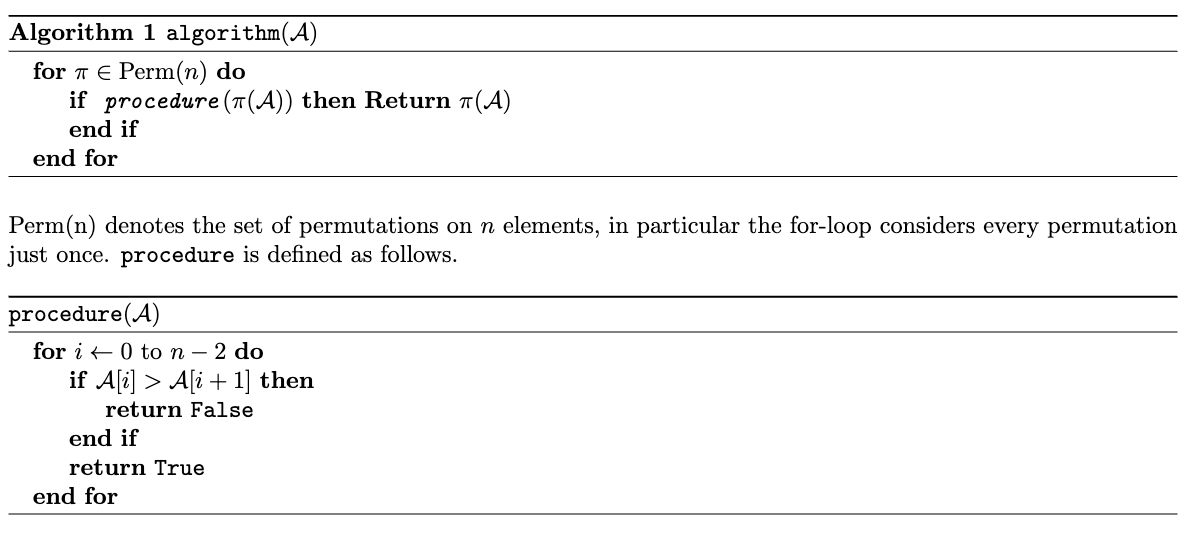
\includegraphics[width=90mm]{02.jpg}
	\caption{Runtime Analysis\label{overflow}}
\end{figure}
\begin{itemize}
	\item What is the output of algorithm1? Explain intermediate steps the algorithm does, in particular proce- dure(A)
	      \begin{itemize}
		      \item The procedure checks if an array is sorted by iterating through each element and checking if it's $\leq$
	      \end{itemize}
	\item What is the runtime of algorithm1? Analyze the worst and the best case
	      \begin{itemize}
		      \item Best runtime: is when the array is already sorted, in which case the runtime is $O(n)$.
		      \item Worst runtime: is when the array is sorted in descending order, in which case the runtime is $O(n^2)$.
	      \end{itemize}
\end{itemize} \section*{Exercise 3: Runtime Analysis} \begin{figure}[ht!] \centering 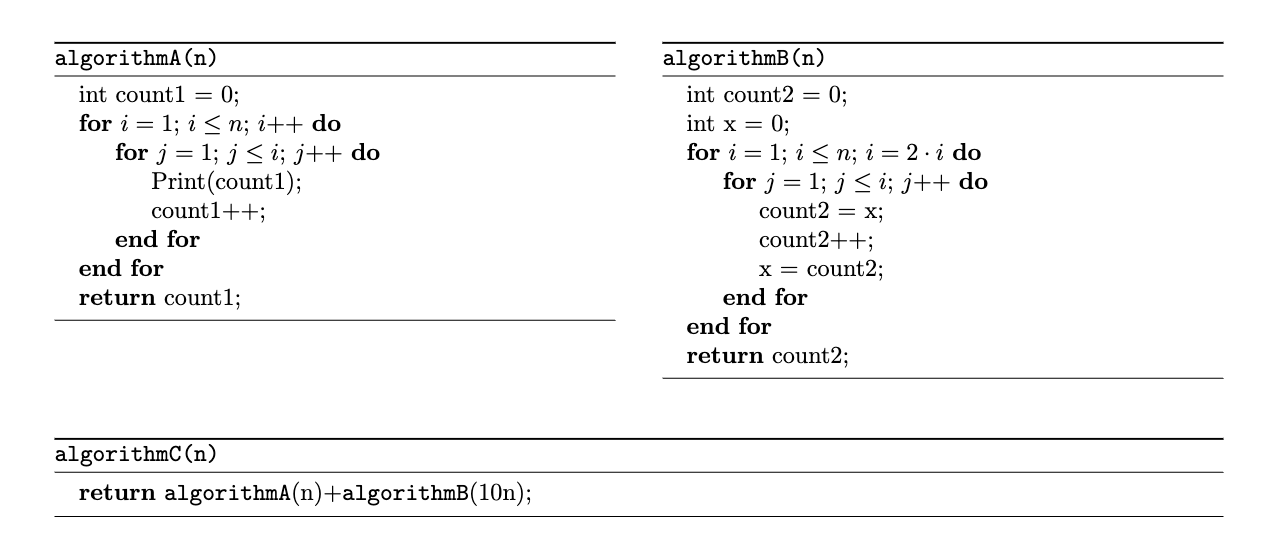
\includegraphics[width=90mm]{03.jpg} \caption{Runtime Analysis\label{overflow}} \end{figure} \begin{itemize} \item What is the output of each of the algorithms? \begin{itemize} \item \textbf{a)} $\frac{n(n+1)}{2}$ \item \textbf{b)} $0$ \\ Always 0, since it's initialized as 0 \item \textbf{c)} $\frac{n(n+1)}{2}$ \\ Since \textbf{Algorithm B(10n)}'s output is always 0 \end{itemize} \item What is the runtime of each of the algorithms? \begin{itemize} \item \textbf{a)} $O(n^2)$ \item \textbf{b)} $O(n)$ \item \textbf{c)} $O(n^2)+O(n)=O(n^2)$ \end{itemize} \end{itemize}

\section*{Exercise 4: \href{https://www.youtube.com/watch?v=x9NhQUxyCpY}{Landau Notation}}

\subsection*{Definition of the O-notation to prove the following}
\subsection*{(a) \( 0.01 \log_c n = \Theta(\ln n) \) for any \( c > 1 \)}

\href{https://www.youtube.com/watch?v=FFm-zaFW_X4}{By change of base formula}, \( \log_c n = \frac{\ln n}{\ln c} \), so \( 0.01 \log_c n = \frac{0.01}{\ln c} \ln n \). Since \( \frac{0.01}{\ln c} \) is a constant, the result follows.

\subsection*{(b) \( \max\{f(n), g(n)\} = \Theta(f(n) + g(n)) \)}
Since \( f(n) \leq f(n) + g(n) \) and \( g(n) \leq f(n) + g(n) \), we have \( \max\{f(n), g(n)\} \leq f(n) + g(n) \). Ergo, \( f(n) + g(n) \leq 2 \max\{f(n), g(n)\} \), proving the claim.

\subsection*{Use the limit criteria to prove the following}

\subsection*{(c) \( (\log_2 n)^2 = \Omega(2^{\log_2 (n^2)}) \)}
Using \( 2^{\log_2 (n^2)} = n^2 \), we need to show \( (\log_2 n)^2 = \Omega(n^2) \). The limit criterion gives:
\[ \lim_{n \to \infty} \frac{(\log_2 n)^2}{n^2} = 0, \]
which contradicts \( \Omega(n^2) \). Thus, the claim is false.

\subsection*{(d) \( 2n^3 + 4n^2 + 7\sqrt{n} = O(n^3) \)}
Taking the limit:
\[ \lim_{n \to \infty} \frac{2n^3 + 4n^2 + 7\sqrt{n}}{n^3} = 2 + \frac{4}{n} + \frac{7\sqrt{n}}{n^3}. \]
Since all terms except 2 vanish as \( n \to \infty \), the function is \( O(n^3) \).

\section*{Exercise 5: Average Runtime of Linear Search}

\end{document}
